\chapter{Estado del arte}
\label{chap:estadodelarte}

\section{Técnicas en bioinformática}

\subsection{Control de calidad}
Las nuevas técnicas de secuenciación masiva proporcionan una gran ventaja en cuanto a la velocidad de lectura de las secuencias~\cite{ngs}. Sin embargo, hay que tener especial precaución en el análisis de la calidad de estas, ya que una mayor velocidad puede llegar a implicar errores en las lecturas en algunos casos. Especialmente, en aquellos en los que se va a realizar un análisis en el que se pueden transmitir estos errores a través de cada una de las herramientas que componen el proceso, pudiendo llegar a provocar conclusiones erróneas al final del análisis.

Uno de los principales factores a tener en cuenta es el método de secuenciación que se haya seguido para obtener las lecturas. Por ejemplo, la tecnología de \textit{Illumina} presenta ciertas complicaciones a raíz de la utilización de adaptadores y primers durante la secuenciación. Al comienzo de ese proceso, durante la preparación de las secuencias, se requiere que se unan a la placa se secuenciación. Para ello, se utilizan adaptadores: cadenas de nucleótidos que se unen a los dos extremos de la secuencia, permitiendo el enlace con los adaptadores complementarios existentes en la placa. Además, para multiplicar el número de secuencias disponibles, se realiza un proceso de PCR, que consiste en replicar las secuencias utilizando polimerasa (la enzima encargada de la replicación y transcripción de ADN). Para que la polimerasa comience este proceso, necesitará reconocer unos patrones concretos en la secuencia de ADN, denominados primers, que deberán haber sido añadidos previamente.

La contaminación con adaptadores y primers utilizados en el proceso de secuenciación, los artefactos (uniones inespecíficas), las lecturas de baja calidad, las inserciones y deleciones son varias de las causas que pueden llevar a análisis problemáticos~\cite{plosone}. No obstante, en la actualidad, existen numerosos métodos enfocados al tratamiento de estos problemas, normalmente agrupados en herramientas entre las que destacan algunas como \textit{FastQC}~\cite{fastqc} o \textit{Prinseq}~\cite{schmieder_prinseq}.

\subsection{Ensamblado}
Los sistemas de secuenciación actuales pierden calidad cuando aumenta el tamaño de las lecturas, por lo tanto, se generan gran cantidad de pequeñas lecturas que deberemos unir. El objetivo del proceso de ensamblado es recoger todos estos fragmentos menores que conformarían una secuencia mayor para alinearlos y empalmarlos con el objetivo de reconstruirla~\cite{assembly_wiki}. Dada la tendencia al aumento de la cantidad de datos a procesar por los ensambladores a raíz de las nuevas técnicas de secuenciación, estos se han visto empujados a emplear técnicas cada vez más eficientes para evitar crear un cuello de botella en esta fase del análisis. Los diferentes aspectos de cada secuenciación como el tamaño, si se trata de un organismo procariota o eucariota, de un transcriptoma, metagenoma, etc, influyen en la eficacia de unos u otros algoritmos. En nuestro caso, al tratarse de bacterias, cuyo genoma es pequeño, se ha decidido utilizar una herramienta destinada a esta característica, como es \textit{SPAdes}~\cite{Nurk2013}. 

Hay que destacar que el problema del ensamblado es, computacionalmente, extremadamente costoso, por lo que la importancia de encontrar un algoritmo que resuelva el problema en un tiempo aceptable es enorme. En este caso, la tecnología en la que se basa tanto esta herramienta como otras muy potentes, como \textit{Velvet}~\cite{Zerbino2008} son los grafos de De Bruijn~\cite{Compeau2011}. Se trata de un tipo de grafos utilizados para representar solapamientos entre secuencias. Es importante tener en cuenta que, en esta representación, los enlaces del grafo estarán formados por las subcadenas de tamaño \textit{k}, denominadas \textit{k-mers} de cada fragmento, mientras que los nodos serán las uniones que utilicen las dos subcadenas para lograr empalmar el final de una con el inicio de la otra, como se aprecia en la figura~\ref{fig:DeBruijn}. La base del algoritmo centrado en este tipo de grafos es encontrar su camino hamiltoniano (que recorra todos los nodos de un grafo una sola vez), siendo este camino la secuencia ensamblada completa.

\begin{figure}
    \begin{center}
      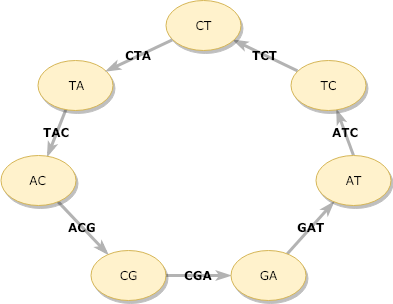
\includegraphics[scale=0.5]{images/DeBruijnGraph.png}
      \caption{Ejemplo de grafo De Bruijn de tamaño de  k-mer 3}
      \label{fig:DeBruijn}
    \end{center}
\end{figure}

\subsection{Anotación}
El proceso de anotación del genoma se basa en identificar y etiquetar todos los aspectos relevantes encontrados en una secuencia, incluyendo, principalmente, regiones codificantes; aunque también son interesantes otros elementos como ARN no codificante, péptidos señal, etc~\cite{RichardsonWatson2012}. 

En algunos casos el proceso se basa en la ejecución de un pipeline automático de anotación seguido de un proceso de filtrado manual~\cite{Stothard2006}. El objetivo en este proyecto es la automatización del proceso en un tiempo de ejecución asequible sin dejar de lado la precisión. En experimentos realizados, \textit{Prokka} ha dado mejores resultados que alternativas como \textit{RAST} o \textit{xBase2} y ha demostrado ser eficiente incluso en ordenadores de usuario con la potencia típica de un PC de sobremesa~\cite{Seemann2014}.

\textit{Prokka}~\cite{Seemann2014} basa su anotación en una serie de herramientas  externas, cada una de ellas especializada en la identificación de una característica de la secuencia concreta, como se explica en la tabla~\ref{table:ProkkaTools}.

\begin{table}[!htb]

\begin{center}
\begin{tabularx}{\textwidth}{bb}
\arrayrulecolor{NavyBlue}\hline
\textbf{\textcolor{NavyBlue}{Herramientas}} &
\textbf{\textcolor{NavyBlue}{Características objetivo}}\\
\quad Prodigal~\cite{Hyatt2010} &
\begin{minipage}[t]{\linewidth}
\quad Secuencias codificantes (CDS)
\end{minipage}\\

\quad RNAmmer~\cite{Lagesen2007} &
\begin{minipage}[t]{\linewidth}
\quad ARN Ribosómico (rRNA)
\end{minipage}\\

\quad Aragorn~\cite{Laslett2004} &
\begin{minipage}[t]{\linewidth}
\quad ARN de transferencia
\end{minipage}\\

\quad SignalP~\cite{Petersen2011} &
\begin{minipage}[t]{\linewidth}
\quad Péptidos señal
\end{minipage}\\

\quad Infernal~\cite{Kolbe2011} &
\begin{minipage}[t]{\linewidth}
\quad ARN no codificante
\end{minipage}\\
\hline
\end{tabularx}
\end{center}
\caption{Herramientas externas de \textit{Prokka}}
\label{table:ProkkaTools}
\end{table}

\subsection{Análisis de resistencia a antibióticos}
Desde el comienzo de la utilización de antibióticos por parte del ser humano, se ha sometido a las bacterias a un proceso de selección natural por el cual aquellas con la capacidad de sobrevivir a cierta concentración de antibiótico, proliferarán. La resistencia a antibióticos se está convirtiendo en uno de los problemas más amenazantes para el ser humano~\cite{Neu1064}. \textit{Campylobacter jejuni}, la bacteria que nos ocupa en este caso, no es una excepción y ya se han detectado casos de resistencia en ella~\cite{Smith1999}. 

Comienzan a identificarse algunos de los genes responsables de esta resistencia y se están creando bases de datos con las que registrarlos~\cite{ARDB}. Consecuentemente, han ido surgiendo herramientas basadas en estas bases de datos con las que contrastar si los fragmentos de cierta secuencia están incluidos en una de ellas. \textit{ABRicate}~\cite{seemann_:mag_right:_2019} es una de las muchas que existen e incluye, tanto bases de datos dedicadas a genes de resistencia a antibióticos como bases de datos de genes de virus.

\subsection{Análisis pangenómico}
El análisis pangenómico en bacterias es un proceso complejo, condicionado siempre a la aparición de nuevos genes. No obstante, su resolución puede suponer ventajas muy significativas~\cite{MEDINI2005589}. Modelos matemáticos aplicados a este problema concluyen que genes únicos continuarán apareciendo independientemente de la cantidad de genomas que se secuencien~\cite{Tettelin13950}. Además, la construcción de este genoma supone un coste computacional muy relevante debido a que se trata de un problema NP-complejo~\cite{Nguyen2015}.

Llegados a este punto, el objetivo en este caso es la construcción de un pangenoma a partir de todas las cepas de las que disponemos y realizar un análisis en el que se indique qué cepas contienen cada gen. En la actualidad se están desarrollando herramientas dedicadas a esta tarea. \textit{Roary}~\cite{Page2015} es una de ellas, basada en la utilización de los fragmentos de secuencias codificantes etiquetados por otras herramientas como \textit{Prokka} para transformarlos en secuencias de proteínas y así simplificar el conjunto de datos. De esta manera, la comparación <<todos contra todos>> de \textit{BLASTP}~\cite{Madden}, se ve muy optimizada.

\section{Herramientas en informática}
Además de las herramientas puramente enfocadas al análisis genético, son necesarias otras técnicas más centradas en la informática para facilitar la utilización del workflow. En este caso, una plataforma con la que poder interactuar con él y un sistema en el que sostener toda su infraestructura.
\subsection{Plataforma de soporte del workflow}
Existe una gran variedad de plataformas sobre las que construir y ejecutar un workflow en la actualidad. Uno de los primeros en aparecer fue \textit{Discovery Net}~\cite{Curcin:2002:DNT:775047.775145}, una utilidad enfocada a coordinar trabajos de servicios ejecutados de manera remota. Sin embargo, es un sistema basado en código y no posee su propia interfaz gráfica, lo que dificultaría su utilización por parte de usuarios ajenos a la programación. Lo mismo ocurre con muchos de los sistemas más utilizados, como \textit{Anduril} \cite{Ovaska2010}, \textit{BioQueue}~ \cite{10.1093/bioinformatics/btx403} o \textit{Cuneiform}~\cite{brandt_reisig_leser_2017}. Sin embargo, hay varios frameworks que permiten un control gráfico del workflow, como \textit{Apache Taverna}~\cite{10.1093/nar/gkt328}, \textit{Triana}~\cite{Taylor2007}, \textit{Kepler}\cite{Ludascher:2006:SWM:1148437.1148454}, \textit{Galaxy}~\cite{Galaxy} o \textit{Yawl}~\cite{yawl2004}. Existen varias publicaciones que analizan las ventajas e inconvenientes de cada uno de los sistemas \cite{4786077, Abouelhoda:2010:MPI:1833398.1833400, Nyronen:2012:DII:2361999.2362006, 10.1093/bib/bbw020}. Entre ellos, por su desarrollo más avanzado y su capacidad para desplegar un sistema completo en un navegador, además de una interfaz fácil de utilizar y una API \textit{Python}~\cite{GalaxyAPI} disponible, destaca \textit{Galaxy}.

\subsection{Virtualización}
Llamamos virtualización a un conjunto de tecnologías destinadas a simular componentes hardware en forma de software. Eso permite la creación de entornos en los que podemos disponer de software y hardware dentro de nuestro propio sistema. Por ejemplo, existe la posibilidad de establecer un sistema \textit{Ubuntu} virtual dentro de un sistema Windows antifrión. En el caso de este ejemplo, estaríamos hablando de una virtualización total, en la que se simula el sistema operativo completo, lo que supone una carga muy pesada debido a que existirá una gran cantidad de software que no va a ser utilizado. En los últimos años se han ido mejorando las técnicas de virtualización parcial, en las que es posible contener solamente la parte mínima de sistema operativo y de software necesarios para la herramienta que queramos simular. Estas técnicas se basan en contenedores, en los que se encapsulan las imágenes con las dependencias necesarias para su funcionamiento. Entre las herramientas más utilizadas, destaca \textit{Docker}~\cite{Docker}, siendo la más reconocida por su popularidad entre los usuarios.

Dado que existe una imagen \textit{Galaxy} estable para \textit{Docker} a partir de la cual poder trabajar, así como una capa adicional desarrollada anteriormente para el mismo grupo de investigación, podemos concluir que \textit{Docker} es el sistema que más se adecúa a las necesidades del proyecto.


\newpage \thispagestyle{empty} % Página vacía 